\documentclass{article}

\usepackage{graphicx}
\usepackage{tikz}
\usepackage{tikzsymbols}
\usetikzlibrary{calc,patterns,shapes.geometric}
\pagestyle{empty}
\usepackage[margin=0pt]{geometry}
\geometry{papersize={14in,12in}}

\def\centerarc[#1](#2)(#3:#4:#5){\draw[#1] ($(#2)+({#5*cos(#3)},{#5*sin(#3)})$) arc (#3:#4:#5);}

\begin{document}
	\begin{figure}
		\centering
		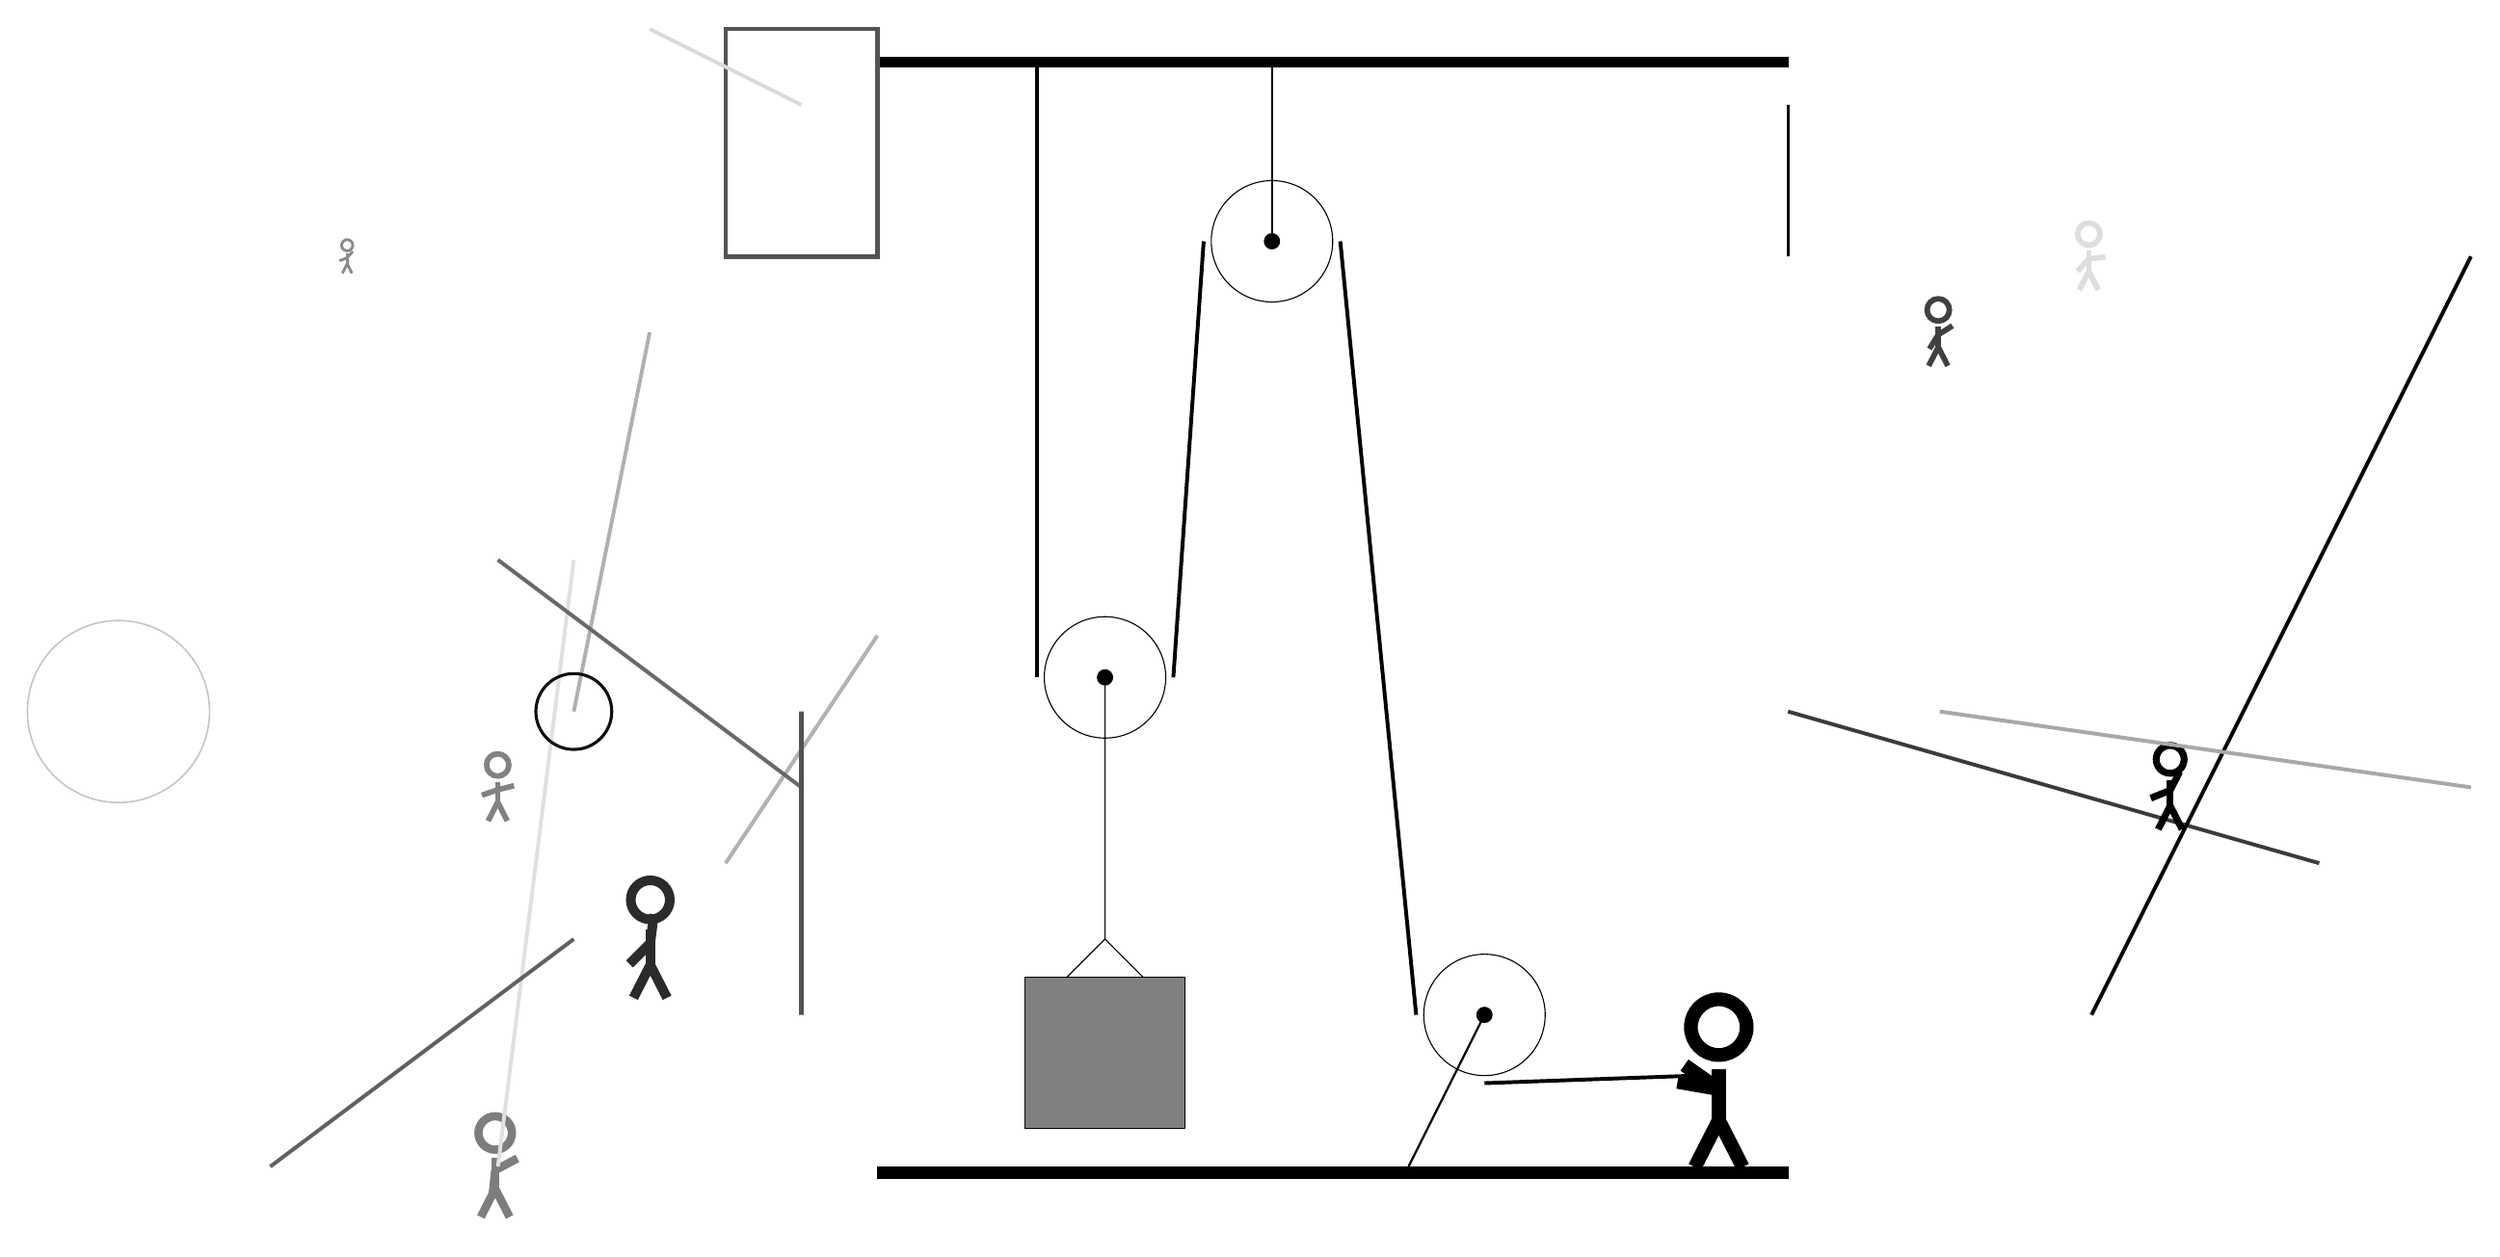
\begin{tikzpicture}
			%%%%% START %%%%%
			
			\draw[fill=black] (-2, 11.5) rectangle (10, 11.625);
			
			\draw (3.2, 9.2) circle (0.8);
			\draw[fill=black] (3.2, 9.2) circle (0.1);
			\draw[thick] (3.2, 9.2) -- (3.2, 11.5);
			
			\draw (6, -1) circle (0.8);
			\draw[fill=black] (6, -1) circle (0.1);
			\draw[thick] (6, -1) -- (5, -3);
			
			\draw[line width=0.6mm, color=black!67] (-4, 12) rectangle (-2, 9);
			
			\draw[line width=0.5mm, color=black!77](10, 3) -- (17, 1);
			\node[line width=0.4mm, color=black!83] at (-5, 0) {\Strichmaxerl[7][45][83]};
			\draw[line width=0.5mm, color=black!31](-5, 8) -- (-6, 3);
			\node[line width=0.3mm, color=black!51] at (-7, -3) {\Strichmaxerl[6][84][28]};
			\node[line width=0.6mm, color=black!13] at (14, 9) {\Strichmaxerl[4][48][7]};
			\draw[line width=0.5mm, color=black!14](-5, 12) -- (-3, 11);
			\node[line width=0.6mm, color=black!100] at (15, 2) {\Strichmaxerl[5][22][63]};
			\draw[line width=0.5mm, color=black!12](-6, 5) -- (-7, -3);
			\draw[line width=0.5mm, color=black!62](-6, 0) -- (-10, -3);
			\node[line width=0.5mm, color=black!75] at (12, 8) {\Strichmaxerl[4][58][32]};
			\draw[line width=0.4mm, color=black!96] (10, 9) rectangle (10, 11);
			\draw[line width=0.5mm, color=black!99](14, -1) -- (19, 9);
			
			\draw [line width=0.2mm, color=black!23](-12, 3) circle (1.2);
			\draw[line width=0.5mm, color=black!34](12, 3) -- (19, 2);
			\draw[line width=0.5mm, color=black!30](-2, 4) -- (-4, 1);
			\draw [line width=0.4mm, color=black!94](-6, 3) circle (0.5);
			\node[line width=0.7mm, color=black!49] at (-7, 2) {\Strichmaxerl[4][19][14]};
			\draw[line width=0.5mm, color=black!59](-3, 2) -- (-7, 5);
			
			\draw[line width=0.6mm, color=black!68] (-3, -1) rectangle (-3, 3);
			\node[line width=0.3mm, color=black!46] at (-9, 9) {\Strichmaxerl[2][23][48]};
			
			
			\draw (1, 3.45) circle (0.8);
			\draw[fill=black] (1, 3.45) circle (0.1);
			
			\draw (1, 3.45) -- (1, 0.0) -- (0.5, -0.5);
			\draw (1, 0.0) -- (1.5, -0.5);
			\draw[fill=black!50] (-0.05, -0.5) rectangle (2.05, -2.5);
			
			\draw[line width=0.5mm] (0.1, 11.5) -- (0.1, 3.45);
			\centerarc[line width=0.5mm](1, 3.45)(180:360:0.9);
			\draw[line width=0.5mm](1.9, 3.45) -- (2.3, 9.2);
			\centerarc[line width=0.5mm](3.2, 9.2)(0:180:0.9);
			\draw[line width=0.5mm](4.1, 9.2) -- (5.1, -1);
			\centerarc[line width=0.5mm](6, -1)(180:270:0.9);
			\draw[line width=0.5mm](6, -1.9) -- (8.8, -1.8);
			
			\node at (9, -1.9) {\Strichmaxerl[10][-35][170]};
			
			\draw[fill=black] (-2, -3) rectangle (10, -3.15);
			
			%%%%% END %%%%%
		\end{tikzpicture}
	\end{figure}	
\end{document}